\documentclass[a4paper,10pt]{ctexart} %ctexart
\usepackage[backref,hidelinks]{hyperref} %hidelinks去掉引用处的红框
\pagestyle{plain} %把页码从右上角移到页脚
%==========打印代码的设置===================
\usepackage{color}
\definecolor{gray}{rgb}{0.8,0.8,0.8}
\usepackage{listings}
\lstset{basicstyle=\small}
\lstset{numbers=left} \lstset{language=C++} \lstset{breaklines}
\lstset{extendedchars=false} \lstset{backgroundcolor=\color{gray}}
\lstset{keywordstyle=\color{blue}\bfseries} \lstset{frame=none}
\lstset{tabsize=4} \lstset{commentstyle=\color{red}}
\lstset{stringstyle=\emph}
%=======================================
%缩小itemize行距
\usepackage{enumitem}
\setenumerate[1]{itemsep=0pt,partopsep=0pt,parsep=\parskip,topsep=5pt}
\setitemize[1]{itemsep=0pt,partopsep=0pt,parsep=\parskip,topsep=5pt}
\setdescription{itemsep=0pt,partopsep=0pt,parsep=\parskip,topsep=5pt}
%=======================================
\begin{document}
\begin{center}
\textbf{AC\_WPNav.cpp}
\end{center}

此文件主要定义了一系列用于实现留待模式(loiter)和航点导航(waypoint navigation)的方法。
首先在构造函数中调用以下两个函数计算用于控制器所需的距离限制参数:
\begin{itemize}
\item calculate\_wp\_leash\_length();\\
计算航点控制器水平和竖直面内的距离限制参数\_wp\_leash\_xy和\_wp\_leash\_z。
对航线上任一点,\_wp\_leash\_xy和\_wp\_leash\_z定义了一个以此点为中心的圆柱体。截面圆位于水平面内,半径是\_wp\_leash\_xy;圆柱高为\_wp\_leash\_z。
将此圆柱体沿航线由起点移动到终点,即得到一个通道。
如果航线位于水平面内,则此通道是一个长度略大于航线长度的长方体,宽和高分别为\_wp\_leash\_xy和\_wp\_leash\_z的2倍;
如果航线位于竖直面内,则此通道是一个高略大于为航线长度的圆柱体,截面圆半径为\_wp\_leash\_z。
对于最一般的情况,此通道是一个斜圆柱。
%wrong!!!:其横截面是矩形,长和宽分别是\_wp\_leash\_xy和\_wp\_leash\_z的两倍。!!!!!!!!!!!!!!!!!!!!!!!!!!!!!!!!!!!!!!!!!!!!
\item calculate\_loiter\_leash\_length();\\
计算目标位置与当前位置的最大距离限制loiter\_leash\_length(水平面内)。
\end{itemize}

AC\_WPNav类的公有成员函数被分为三部分:\\
1) simple loiter controller, 用于实现留待模式;\\
2) waypoint controller, 用于实现航点控制;\\
3) shared methods, 两种控制通用的方法。\\
核心为两个控制器函数:1)中的update\_loiter()和2)中的update\_wpnav(),应以10Hz速率被调用。
另有一系列protected成员函数被公有成员函数调用(除get\_bearing\_cd()外其余都是被某个/两个控制器函数调用)。

两个控制器都利用switch结构将控制过程分为4步,每步调用相应的函数:\\
\textbf{update\_loiter()留待控制器}:\\
1.translate\_loiter\_target\_movements(\_loiter\_dt);\\
2.get\_loiter\_position\_to\_velocity(\_loiter\_dt, WPNAV\_...\_ERROR);\\
3.get\_loiter\_velocity\_to\_acceleration(desired\_vel.x, desired\_vel.y, \_loiter\_dt);\\
4.get\_loiter\_acceleration\_to\_lean\_angles(desired\_accel.x, desired\_accel.y);

\noindent\textbf{update\_wpnav()航点控制器}:\\
1.advance\_target\_along\_track(dt);\\
2.get\_loiter\_position\_to\_velocity(\_wpnav\_dt, \_wp\_speed\_cms);\\
3.get\_loiter\_velocity\_to\_acceleration(desired\_vel.x, desired\_vel.y, \_wpnav\_dt);\\
4.get\_loiter\_acceleration\_to\_lean\_angles(desired\_accel.x, desired\_accel.y);\\
(说明:\\
1.留待控制器不涉及高度通道的控制。\\
2.航点控制器只实现航点导航的最基础部分,即两航点之间的直线导航。
故下面提到的“航线”是两航点之间的直线段而不是实际飞行中的复杂航线,“起点”和“终点”是这一线段的两个端点而不是实际飞行任务的起点和终点)。

两个控制器第1步调用的函数用于更新\_target。
对于留待控制器,\_target是留待目标点;对于航点控制器,\_target是中间点。
(中间点可理解为飞行器在起点到终点的飞行过程中,某时刻飞行器的实际位置在航线上的投影点,用以表征飞行器沿航线飞行的进度。)
2-4步两个控制器调用了相同的函数,
get\_loiter\_position\_to\_velocity()由位置误差求解速度修正量,进而得到速度的目标值;
get\_loiter\_velocity\_to\_acceleration()使用PID控制器,由速度误差求解加速度修正量,然后与前馈加速度相加得到加速度的目标值;
get\_loiter\_acceleration\_to\_lean\_angles()利用重力加速度和机体系目标加速度的几何关系,求解飞行器的倾斜角。


%==============simple loiter controller==============
下面按照此cpp文件定义函数的顺序分析各函数,略去简单函数。

\vspace{10pt}
\noindent \textbf{\large 1)simple loiter controller部分的函数:}

\noindent get\_stopping\_point(const Vector3f\& position, const Vector3f\& velocity, Vector3f \&target) {\color{red}*116}\\
利用水平位置和速度信息计算目标点位置target,目标点到当前位置距离不超过\_wp\_leash\_xy。此函数被set\_destination()调用。\\
1.计算当前速度。如果速度小于10cm/s,kP很小或加速度为零,直接将目标位置设置为当前位置。
\begin{lstlisting}
    vel_total = safe_sqrt(velocity.x*velocity.x + velocity.y*velocity.y);
    if (vel_total < 10.0f || kP <= 0.0f || _wp_accel_cms <= 0.0f) {
        target = position;
        return;
    }
\end{lstlisting}
2.计算目标位置距当前位置的距离target\_dist。定义了一个以当前速度vel\_total为自变量的分段函数,速度小于临界速度时距离是当前速度的线性函数,大于临界速度时距离是当前速度的二次函数:
\begin{lstlisting}
    //计算分段函数的临界点
    linear_velocity = _wp_accel_cms/kP;
    if (vel_total < linear_velocity) {
        target_dist = vel_total/kP;
    } else {
        linear_distance = _wp_accel_cms/(2.0f*kP*kP);
        target_dist = linear_distance + (vel_total*vel_total)/(2.0f*_wp_accel_cms);
    }
    //对求得的距离进行限幅,不能超过航点控制器水平方向的距离限制_wp_leash_xy
    target_dist = constrain_float(target_dist, 0, _wp_leash_xy);
\end{lstlisting}
3.由当前位置和上一步求得的距离计算目标位置。
\begin{lstlisting}
    target.x = position.x + (target_dist * velocity.x / vel_total);
    target.y = position.y + (target_dist * velocity.y / vel_total);
    target.z = position.z;
\end{lstlisting}


\vspace{8pt}
\noindent set\_loiter\_target(const Vector3f\& position)\\
设置留待目标位置,并将目标速度\_target\_vel置零。

\vspace{8pt}
\noindent init\_loiter\_target(const Vector3f\& position, const Vector3f\& velocity)\\
初始化目标点。\\
1.将留待目标位置和目标速度设置为当前位置和速度。
\begin{lstlisting}
    _target.x = position.x;
    _target.y = position.y;
    _target_vel.x = velocity.x;
    _target_vel.y = velocity.y;
\end{lstlisting}
2.将滚转角和俯仰角的目标值\_desired\_roll和\_desired\_pitch设置为当前实际角度,防止初次运行留待控制器时发生颤动。
\begin{lstlisting}
    _desired_roll = constrain_int32(_ahrs->roll_sensor,-_lean_angle_max_cd,_lean_angle_max_cd);
    _desired_pitch = constrain_int32(_ahrs->pitch_sensor,-_lean_angle_max_cd,_lean_angle_max_cd);
\end{lstlisting}
3.将由遥控输入量计算得到的速度\_pilot\_vel\_forward\_cms和\_pilot\_vel\_right\_cms置零。\\
4.将\_vel\_last设置为当前的速度。
\begin{lstlisting}
    _vel_last = _inav->get_velocity();	
\end{lstlisting}

\vspace{8pt}
\noindent move\_loiter\_target(float control\_roll, float control\_pitch, float dt)\\
将遥控输入量转换为向前和向右的速度\_pilot\_vel\_forward\_cms和\_pilot\_vel\_right\_cms,下面称为机体系遥控目标速度。
\begin{lstlisting}
    _pilot_vel_forward_cms = -control_pitch * _loiter_accel_cms / 4500.0f;
    _pilot_vel_right_cms = control_roll * _loiter_accel_cms / 4500.0f;
\end{lstlisting}

\vspace{8pt}
\noindent translate\_loiter\_target\_movements(float nav\_dt){\color{red}*188}\\
由上一个函数move\_loiter\_target()的输出量\_pilot\_vel\_forward\_cms和\_pilot\_vel\_right\_cms求解目标位置\_target。\\
1.将机体系遥控目标速度\_pilot\_vel\_forward\_cms和\_pilot\_vel\_right\_cms转换到惯性系得到速度调整量target\_vel\_adj:
\begin{lstlisting}
    target_vel_adj.x = (_pilot_vel_forward_cms*_cos_yaw - _pilot_vel_right_cms*_sin_yaw);
    target_vel_adj.y = (_pilot_vel_forward_cms*_sin_yaw + _pilot_vel_right_cms*_cos_yaw);
\end{lstlisting}
2.将速度调整量添加到当前的惯性系遥控目标速度中:
\begin{lstlisting}
    _target_vel.x += target_vel_adj.x*nav_dt;
    _target_vel.y += target_vel_adj.y*nav_dt;
\end{lstlisting}
3.对惯性系遥控目标速度进行处理,原理不清楚???
\begin{lstlisting}
    if(_target_vel.x > 0 ) {
        _target_vel.x -= (_loiter_accel_cms-WPNAV_LOITER_ACCEL_MIN)*nav_dt*_target_vel.x/_loiter_speed_cms;
        _target_vel.x = max(_target_vel.x - WPNAV_LOITER_ACCEL_MIN*nav_dt, 0);
        ……
\end{lstlisting}
4.对惯性系遥控目标速度向量进行限幅:
\begin{lstlisting}
    vel_total = safe_sqrt(_target_vel.x*_target_vel.x + _target_vel.y*_target_vel.y);
    if (vel_total > _loiter_speed_cms && vel_total > 0.0f) {
        _target_vel.x = _loiter_speed_cms * _target_vel.x/vel_total;
        _target_vel.y = _loiter_speed_cms * _target_vel.y/vel_total;
    }
\end{lstlisting}
5.更新目标位置。如果其距当前位置的距离超出\_loiter\_leash限制,则进行限幅处理,将目标位置限制到以curr\_pos为圆心,\_loiter\_leash为半径的圆上:
\begin{lstlisting}
    _target.x += _target_vel.x * nav_dt;
    _target.y += _target_vel.y * nav_dt;
    Vector3f curr_pos = _inav->get_position();
    Vector3f distance_err = _target - curr_pos;
    float distance = safe_sqrt(distance_err.x*distance_err.x + distance_err.y*distance_err.y);
    if (distance > _loiter_leash && distance > 0.0f) {
        _target.x = curr_pos.x + _loiter_leash * distance_err.x/distance;
        _target.y = curr_pos.y + _loiter_leash * distance_err.y/distance;
    }
\end{lstlisting}

\vspace{8pt}
\noindent update\_loiter()\\
留待控制器,见前面。

\vspace{8pt}
\noindent calculate\_loiter\_leash\_length() {\color{red}*308}\\
计算目标位置可能距当前位置的距离的最大值。类似前面get\_stopping\_point()函数,定义了一个分段函数。
\begin{lstlisting}
    // 将留待加速度设置为留待速度的一半
    _loiter_accel_cms = _loiter_speed_cms / 2.0f;
    if(WPNAV_LOITER_SPEED_MAX_TO_CORRECT_ERROR <= _wp_accel_cms / kP) {
        _loiter_leash = WPNAV_LOITER_SPEED_MAX_TO_CORRECT_ERROR / kP;
    }else{
        _loiter_leash = (_wp_accel_cms / (2.0f*kP*kP)) + (WPNAV_LOITER_SPEED_MAX_TO_CORRECT_ERROR*WPNAV_LOITER_SPEED_MAX_TO_CORRECT_ERROR / (2.0f*_wp_accel_cms));
    }
    // 确保_loiter_leash长度至少1m
    if( _loiter_leash < WPNAV_MIN_LEASH_LENGTH ) {
        _loiter_leash = WPNAV_MIN_LEASH_LENGTH;
\end{lstlisting}



\vspace{20pt}
%==================waypoint controller==============
\noindent \textbf{\large 2)waypoint controller部分的函数:}

\noindent set\_destination(const Vector3f\& destination)\\
1.设置起点\_origin:如果启用了航点控制器且飞行器抵达了上一个航点,则将其设置为新一段航线的起点\_origin;否则,调用get\_stopping\_point()计算\_origin()。
\begin{lstlisting}
    // if waypoint controlls is active and copter has reached the previous waypoint use it for the origin
    if( _flags.reached_destination && ((hal.scheduler->millis() - _wpnav_last_update) < 1000) ) {
        _origin = _destination;
    }else{
        // otherwise calculate origin from the current position and velocity
        get_stopping_point(_inav->get_position(), _inav->get_velocity(), _origin);
    }
\end{lstlisting}
2.调用set\_origin\_and\_destination(\_origin, destination)设置起点和终点。起点上一步已设置,这里重复设置没意义,只是为了把\_origin传进函数进行相关的计算。

\vspace{8pt}
\noindent set\_origin\_and\_destination(const Vector3f\& origin, const Vector3f\& destination){\color{red}*361}\\
设置起点和终点,并初始化一系列参数。\\
1.设置起点和终点,计算两点间向量的距离,并得到其单位方向向量。
\begin{lstlisting}
    _origin = origin;
    _destination = destination;
    Vector3f pos_delta = _destination - _origin;
    _track_length = pos_delta.length(); 
    _pos_delta_unit = pos_delta/_track_length;
\end{lstlisting}
2.计算航点控制器的限制长度。注意由于speed\_up\_cms和speed\_down\_cms不同,爬升和下降时的限制长度不同。
\begin{lstlisting}
    bool climb = pos_delta.z >= 0;
    calculate_wp_leash_length(climb); 
\end{lstlisting}
3将中间点\_target初始化在起点。(中间点可理解为飞行器在起点到终点的飞行过程中,某时刻飞行器的实际位置在航线上的投影点,用以表征飞行器沿航线飞行的进度。)
\begin{lstlisting}
    _track_desired = 0;
    _target = origin;
    _flags.reached_destination = false;
\end{lstlisting}
4.将中间点的速度\_limited\_speed\_xy\_cms初始化为当前速度在航线方向的分量,并限幅在最大水平速度\_wp\_speed\_cms下。
\begin{lstlisting}
    const Vector3f &curr_vel = _inav->get_velocity();
    float speed_along_track = curr_vel.x * _pos_delta_unit.x + curr_vel.y * _pos_delta_unit.y + curr_vel.z * _pos_delta_unit.z;
    _limited_speed_xy_cms = constrain_float(speed_along_track,0,_wp_speed_cms);
\end{lstlisting}
5.其余操作:设置非快速航点模式,将滚转角和俯仰角的目标值\_desired\_roll和\_desired\_pitch设置为当前实际角度,将目标速度置零。
\begin{lstlisting}
    _flags.fast_waypoint = false;
    _desired_roll = constrain_int32(_ahrs->roll_sensor,-_lean_angle_max_cd,_lean_angle_max_cd);
    _desired_pitch = constrain_int32(_ahrs->pitch_sensor,-_lean_angle_max_cd,_lean_angle_max_cd);
    _target_vel.x = 0;
    _target_vel.y = 0;
\end{lstlisting}

\vspace{8pt}
\noindent advance\_target\_along\_track(float dt){\color{red}*408}\\
沿航线将中间点\_target由起点向终点移动。\\
1.获得当前位置curr\_pos、起点指向当前位置的向量curr\_delta、沿航线已经飞过的距离track\_covered和航迹误差向量track\_error(当前位置到航线的垂直距离)。计算航迹误差在水平和竖直方向上的分量track\_error\_xy和track\_error\_z。
\begin{lstlisting}
    Vector3f curr_pos = _inav->get_position();
    Vector3f curr_delta = curr_pos - _origin;
    track_covered = curr_delta.x * _pos_delta_unit.x + curr_delta.y * _pos_delta_unit.y + curr_delta.z * _pos_delta_unit.z;
    Vector3f track_covered_pos = _pos_delta_unit * track_covered;
    track_error = curr_delta - track_covered_pos;
    float track_error_xy = safe_sqrt(track_error.x*track_error.x + track_error.y*track_error.y);
    float track_error_z = fabsf(track_error.z);
\end{lstlisting}
2.计算在\_wp\_leash\_xy和\_wp\_leash\_z限制范围内,中间点距起点的距离的最大允许值track\_desired\_max。
\_track\_leash\_length是沿航线方向的限制长度。

% 不确定下面的分析对不对。。
分析计算公式的原理,考虑一种简单情况,如图\ref{advancetargetalongtrack}所示。
假设航线沿竖直方向,则不存在track\_error\_z。
通道为一圆柱体,截面圆半径为\_wp\_leash\_xy。作另一截面圆半径为track\_error\_xy的圆柱体,当前位置在其侧表面上。
根据当前位置的误差情况来决定本次函数执行中,中间点向前移动的最大距离:当前的位置误差越大,则track\_extra\_max越小;
当当前位置恰好处于航线上即位置误差为0时,track\_extra\_max取得最大值即\_track\_leash\_length。
\begin{figure}[!htb]\center
\includegraphics[scale=0.4]{advance_target_along_track.png}
\caption{advance\_target\_along\_track}\label{advancetargetalongtrack}
\end{figure}

%wrong!!!:\_wp\_leash\_xy和\_wp\_leash\_z的限制范围是一个以航线为中心的管道,横截面是矩形,其长和宽分别是\_wp\_leash\_xy和\_wp\_leash\_z的两倍。
%看不懂计算track\_extra\_max的公式的物理意义???
%如果\_wp\_leash\_xy(\_z)是水平(竖直)面内垂直于航线的距离限制的话,利用三角形相似,
%min()的参数应该是track\_covered/(\_wp\_leash\_X-track\_error\_X/\_wp\_leash\_X,X表示xy和z。(codeline433)
%没有超出限制范围后进行修正的代码???????再分析一下track\_leash\_length的作用?????????????????????????????????????????????
%????????????????????????????????????????????????????????????????????????????????????????????????????????????????????????
\begin{lstlisting}
    track_extra_max = min(_track_leash_length*(_wp_leash_z-track_error_z)/_wp_leash_z, _track_leash_length*(_wp_leash_xy-track_error_xy)/_wp_leash_xy);
    if(track_extra_max <0) {
        track_desired_max = track_covered;
    }else{
        track_desired_max = track_covered + track_extra_max;
    }
\end{lstlisting}
3.得到当前速度和其在航线上的分量speed\_along\_track。设置一个速度阈值linear\_velocity,根据speed\_along\_track与速度阈值的关系,对中间点速度进行相应的处理,将其限制在speed\_along\_track上下一定范围内。
\begin{lstlisting}
    const Vector3f &curr_vel = _inav->get_velocity();
    float speed_along_track = curr_vel.x * _pos_delta_unit.x + curr_vel.y * _pos_delta_unit.y + curr_vel.z * _pos_delta_unit.z;
    ……
    linear_velocity = _track_accel/kP;
    if (speed_along_track < -linear_velocity) {
        //飞行方向与航线方向相反,则不移动中间点,即中间点速度为0
        _limited_speed_xy_cms = 0;
    }else{
    		//中间点距起点的距离未达到最大允许值,即飞行器距航线的距离仍在限制范围内,则提速
            if(track_desired_max > _track_desired) {
                _limited_speed_xy_cms += 2.0f * _track_accel * dt;
            }else{
                // 中间点距起点的距离超出了最大允许值,即飞行器超出了限制范围,则不再提速
                _track_desired = track_desired_max;
            }
        }
        // 中间点速度最大不超过_track_speed
        if(_limited_speed_xy_cms > _track_speed) {
            _limited_speed_xy_cms = _track_speed;
        }
        // 如果当前速度在航线上的分量在速度阈值范围内,则将中间点的速度限制在speed_along_track上下一定范围内。目的是防止飞行器经过一个航点后产生过大的加速度
        if (fabsf(speed_along_track) < linear_velocity) {
            _limited_speed_xy_cms = constrain_float(_limited_speed_xy_cms,speed_along_track-linear_velocity,speed_along_track+linear_velocity);
        }
    }
\end{lstlisting}
4.更新中间点位置。\_track\_desired是中间点距起点的距离,track\_desired\_temp通过积分中间点的速度以获得此值。\_track\_length是起点到终点的距离。
\begin{lstlisting}
    track_desired_temp += _limited_speed_xy_cms * dt;

    // do not let desired point go past the end of the segment
    track_desired_temp = constrain_float(track_desired_temp, 0, _track_length);
    _track_desired = max(_track_desired, track_desired_temp);

    _target = _origin + _pos_delta_unit * _track_desired;
\end{lstlisting}
5.检查是否已经抵达终点。
\begin{lstlisting}
   if( !_flags.reached_destination ) {
   //快速航点模式下,中间点抵达终点即认为航线已完成
        if( _track_desired >= _track_length ) {
            if (_flags.fast_waypoint) {
    		    _flags.reached_destination = true;
            }else{
                //非快速航点模式下,除中间点抵达终点外,还要求飞行器位于以终点为圆心的某个圆域内
                Vector3f dist_to_dest = curr_pos - _destination;
                if( dist_to_dest.length() <= _wp_radius_cm ) {
                    _flags.reached_destination = true;
                }
            }
        }
    }
\end{lstlisting}


\vspace{8pt}
\noindent get\_distance\_to\_destination()\\
使用惯导系统获得当前位置,然后计算距终点的水平距离。

\vspace{8pt}
\noindent get\_bearing\_to\_destination()\\
计算终点的方位角。

\vspace{8pt}
\noindent update\_wpnav()\\
航点控制器,见前面。

\vspace{20pt}
\noindent \textbf{\large 3)shared methods部分的函数:}

\noindent get\_loiter\_position\_to\_velocity(float dt, float max\_speed\_cms)\\
根据目标位置和当前位置计算速度的目标值。

\begin{figure}[!htb]\center
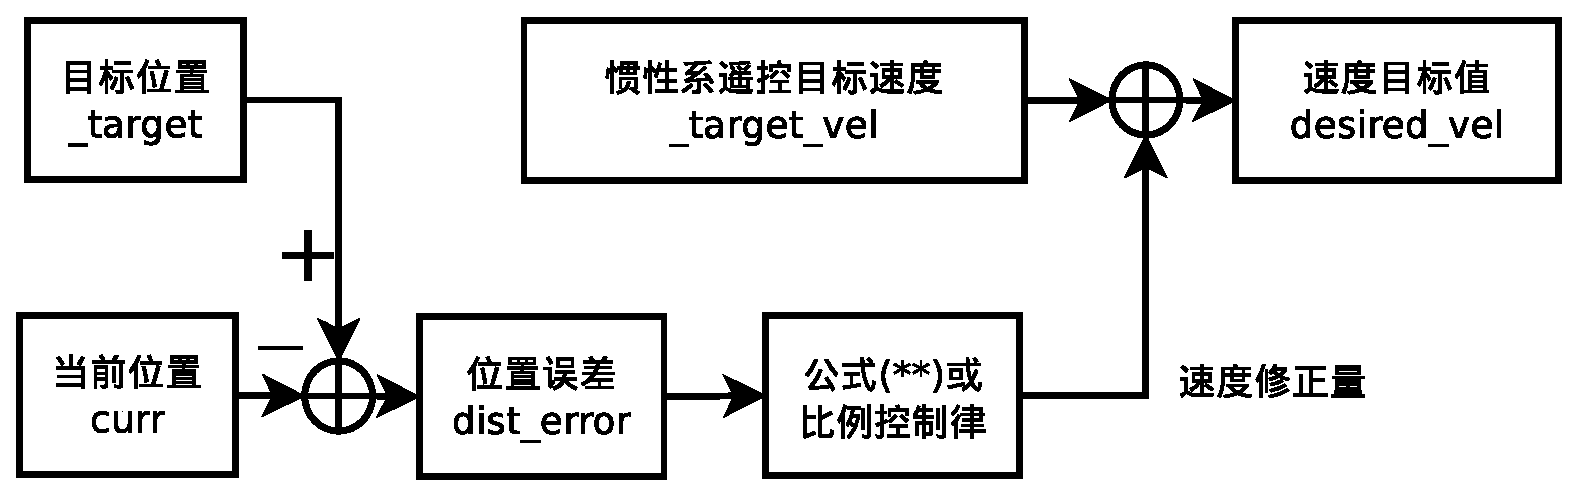
\includegraphics[scale=0.3]{get_loiter_position_to_velocity.eps}
\caption{get\_loiter\_position\_to\_velocity}\label{getloiterpositiontovelocity}
\end{figure}
1.计算位置误差,并定义一个误差距离阈值linear\_distance,将在下面计算速度修正量时使用。
\begin{lstlisting}
        dist_error.x = _target.x - curr.x;
        dist_error.y = _target.y - curr.y;
        linear_distance = _wp_accel_cms/(2.0f*kP*kP);
        dist_error_total = safe_sqrt(dist_error.x*dist_error.x + dist_error.y*dist_error.y);
\end{lstlisting}
2.计算速度修正量。如果距离误差大于距离阈值的两倍,则按照式(**)求解修正量;否则,使用比例控制律。
即,修正量计算公式为以距离误差为自变量的连续分段函数,分界点为(2linear\_distance,\_wp\_accel\_cms/kP),
分界点前修正量线性增长,分界点后修正量以平方根规律增长。
\begin{lstlisting}
        if( dist_error_total > 2.0f*linear_distance ) {
            vel_sqrt = safe_sqrt(2.0f*_wp_accel_cms*(dist_error_total-linear_distance)); //**
            desired_vel.x = vel_sqrt * dist_error.x/dist_error_total;
            desired_vel.y = vel_sqrt * dist_error.y/dist_error_total;
        }else{
            desired_vel.x = _pid_pos_lat->kP() * dist_error.x;
            desired_vel.y = _pid_pos_lon->kP() * dist_error.y;
        }
\end{lstlisting}
3.对速度修正量进行限幅。
\begin{lstlisting}
        vel_total = safe_sqrt(desired_vel.x*desired_vel.x + desired_vel.y*desired_vel.y);
        if( vel_total > max_speed_cms ) {
            desired_vel.x = max_speed_cms * desired_vel.x/vel_total;
            desired_vel.y = max_speed_cms * desired_vel.y/vel_total;
        }
\end{lstlisting}
4.将速度修正量和惯性系遥控目标速度(由遥控输入量计算得到的速度)相加,得到最终速度的目标值。
\begin{lstlisting}
        desired_vel.x += _target_vel.x;	
        desired_vel.y += _target_vel.y;
\end{lstlisting}
\vspace{8pt}
\noindent get\_loiter\_velocity\_to\_acceleration(float vel\_lat, float vel\_lon, float dt)\\
根据速度信息计算加速度的目标值。结果由两部分组成:前馈加速度和反馈通道PID控制器的输出量(即加速度的修正量)。

\begin{figure}[!htb]\center
\includegraphics[scale=0.3]{get_loiter_velocity_to_acceleration.eps}
\caption{get\_loiter\_velocity\_to\_acceleration}\label{getloitervelocitytoacceleration}
\end{figure}
1.计算前馈加速度。
\begin{lstlisting}
        desired_accel.x = (vel_lat - _vel_last.x)/dt;
        desired_accel.y = (vel_lon - _vel_last.y)/dt;
\end{lstlisting}
2.计算最终加速度的目标值。先计算速度误差,然后将其输入PID控制器得到加速度的修正量,与前馈加速度相加得到最终加速度的目标值。
\begin{lstlisting}
    // calculate velocity error
    vel_error.x = vel_lat - vel_curr.x;
    vel_error.y = vel_lon - vel_curr.y;
    // combine feed foward accel with PID output from velocity error
    desired_accel.x += _pid_rate_lat->get_pid(vel_error.x, dt);
    desired_accel.y += _pid_rate_lon->get_pid(vel_error.y, dt);
\end{lstlisting}
3.限幅处理。
\begin{lstlisting}
    accel_total = safe_sqrt(desired_accel.x*desired_accel.x + desired_accel.y*desired_accel.y);
    if( accel_total > WPNAV_ACCEL_MAX ) {
        desired_accel.x = WPNAV_ACCEL_MAX * desired_accel.x/accel_total;
        desired_accel.y = WPNAV_ACCEL_MAX * desired_accel.y/accel_total;
    }
\end{lstlisting}

\vspace{8pt}
\noindent get\_loiter\_acceleration\_to\_lean\_angles(float accel\_lat, float accel\_lon)\\
由目标加速度求解飞行器的倾斜角。先将目标加速度转换到机体系,然后利用重力加速度和机体系目标加速度的几何关系求得飞行器的倾斜角。
\begin{eqnarray}
\phi	& = & arctan{\frac{accel\_right\cdot cos\theta}{g}}\\ \nonumber
\theta	& = & arctan{\frac{-accel\_forward}{g}}
\end{eqnarray}
\begin{lstlisting}
    //gravity in cm/s/s
    float z_accel_meas = -GRAVITY_MSS * 100;
    // rotate accelerations into body forward-right frame
    accel_forward = accel_lat*_cos_yaw + accel_lon*_sin_yaw;
    accel_right = -accel_lat*_sin_yaw + accel_lon*_cos_yaw;
    // update angle targets that will be passed to stabilize controller
    _desired_roll = constrain_float(fast_atan(accel_right*_cos_pitch/(-z_accel_meas))*(18000/M_PI_F), -_lean_angle_max_cd, _lean_angle_max_cd);
    _desired_pitch = constrain_float(fast_atan(-accel_forward/(-z_accel_meas))*(18000/M_PI_F), -_lean_angle_max_cd, _lean_angle_max_cd);
\end{lstlisting}

\vspace{8pt}
\noindent get\_bearing\_cd(const Vector3f \&origin, const Vector3f \&destination)\\
计算方位角。此函数在数学库中也实现过。
\begin{lstlisting}
    float bearing = 9000 + atan2f(-(destination.x-origin.x), destination.y-origin.y) * 5729.57795f;
\end{lstlisting}
函数原型为atan2(y,x),注意此处坐标系是x向上y向右(North-East),故atan参数中x在前。
x,y都为正时,atan2得到的角度介于(-PI/2,0),等于bearing的余角的相反数,加90度得到方位角。

\vspace{8pt}
\noindent reset\_I()\\
清零PID控制器的积分项。并将\_vel\_last设置为当前速度。

\vspace{8pt}
\noindent calculate\_wp\_leash\_length(bool climb) {\color{red}*700}\\
计算航点控制器的距离限制限制参数\_wp\_leash\_xy和\_wp\_leash\_z。\\
1.计算水平方向的距离限制。定义了一个关于\_wp\_speed\_cms的连续分段函数,分段点为(\_wp\_accel\_cms/kP,\_wp\_speed\_cms/kP),
分段点前\_wp\_leash\_xy为常值,分段点后呈平方率增长。
\begin{lstlisting}
    if(_wp_speed_cms <= _wp_accel_cms / kP) {
        // linear leash length based on speed close in
        _wp_leash_xy = _wp_speed_cms / kP;
    }else{
        // leash length grows at sqrt of speed further out
        _wp_leash_xy = (_wp_accel_cms / (2.0f*kP*kP)) + (_wp_speed_cms*_wp_speed_cms / (2.0f*_wp_accel_cms));
    // ensure leash is at least 1m long
    if( _wp_leash_xy < WPNAV_MIN_LEASH_LENGTH ) {
        _wp_leash_xy = WPNAV_MIN_LEASH_LENGTH;
    }
\end{lstlisting}
在全局范围内搜索\_wp\_speed\_cms和\_wp\_accel\_cms,其只在初始化时被赋值,之后未被修改过,因此PID参数kP确定后
\_wp\_leash\_xy是常值。\\
2.计算竖直方向的距离限制。类似第1步,定义了一个关于竖直方向速度speed\_vert的连续分段函数。
\begin{lstlisting}
    float speed_vert;
    if( climb ) {
        speed_vert = _wp_speed_up_cms;	///250
    }else{
        speed_vert = _wp_speed_down_cms;///150
    }
    if(speed_vert <= WPNAV_ALT_HOLD_ACCEL_MAX / _althold_kP) {	///WPNAV_ALT_HOLD_ACCEL_MAX=250
        // linear leash length based on speed close in
        _wp_leash_z = speed_vert / _althold_kP;
    }else{
        // leash length grows at sqrt of speed further out
        _wp_leash_z = (WPNAV_ALT_HOLD_ACCEL_MAX / (2.0*_althold_kP*_althold_kP)) + (speed_vert*speed_vert / (2*WPNAV_ALT_HOLD_ACCEL_MAX));
    }
    // ensure leash is at least 1m long
    if( _wp_leash_z < WPNAV_MIN_LEASH_LENGTH ) {
        _wp_leash_z = WPNAV_MIN_LEASH_LENGTH;
    }
\end{lstlisting}
3.计算沿航线方向的加速度、速度和限制长度\_track\_leash\_length。
\begin{lstlisting}
    // length of the unit direction vector in the horizontal
    float pos_delta_unit_xy = sqrt(_pos_delta_unit.x*_pos_delta_unit.x+_pos_delta_unit.y*_pos_delta_unit.y);
    float pos_delta_unit_z = fabsf(_pos_delta_unit.z);

    if(pos_delta_unit_z == 0 && pos_delta_unit_xy == 0){
        _track_accel = 0;
        _track_speed = 0;
        _track_leash_length = WPNAV_MIN_LEASH_LENGTH;	///100
    }else if(_pos_delta_unit.z == 0){
        _track_accel = _wp_accel_cms/pos_delta_unit_xy;
        _track_speed = _wp_speed_cms/pos_delta_unit_xy;
        _track_leash_length = _wp_leash_xy/pos_delta_unit_xy;
    }else if(pos_delta_unit_xy == 0){
        _track_accel = WPNAV_ALT_HOLD_ACCEL_MAX/pos_delta_unit_z;
        _track_speed = speed_vert/pos_delta_unit_z;
        _track_leash_length = _wp_leash_z/pos_delta_unit_z;
    }else{
        _track_accel = min(WPNAV_ALT_HOLD_ACCEL_MAX/pos_delta_unit_z, _wp_accel_cms/pos_delta_unit_xy);
        _track_speed = min(speed_vert/pos_delta_unit_z, _wp_speed_cms/pos_delta_unit_xy);
        _track_leash_length = min(_wp_leash_z/pos_delta_unit_z, _wp_leash_xy/pos_delta_unit_xy);
    }
\end{lstlisting}


\begin{flushright}
\vspace{10pt}
2015.8.13\\
方酉
\end{flushright}
\end{document}